\chapter{Phạm vi và hướng phát triển ứng dụng webfuzzer}
Chương này so sánh \textbf{webfuzzer} với các công cụ, dịch vụ và khung thức kiểm thử hiện đang được sử dụng trong cộng đồng.\par
Trong phạm vi luận văn tốt nghiệp này, tôi sẽ áp dụng phương pháp kiểm thử fuzzing dưới dạng kiểm thử hộp đen để hiện thực công cụ \textbf{webfuzzer}. Ngoài khả năng tự động hóa cao, việc áp dụng phương pháp này sẽ đem lại nhiều lợi ích khác.
\begin{itemize}
    \item Linh hoạt trong việc kiểm thử nhiều ứng dụng web sử dụng các công nghệ, mô hình, khung thức phát triển phần mềm khác nhau, cũng như cho phép kiểm thử số lượng lớn ứng dụng web trong một khoảng thời gian ngắn.
    \item Đơn giản hóa và chuẩn hóa việc kiểm thử các lỗ hổng bảo mật trên những ứng dụng web có thiết kế cao cấp và phức tạp. Những ứng dụng này thường có số lượng dòng code có thể lên đến hàng nghìn thậm chí hàng triệu dòng, việc kiểm thử mã nguồn đối với phương pháp hộp trắng hoặc hộp xám sẽ khó khăn hơn nhiều.
    \item Dễ dàng đạt được khả năng tự động hóa cao so với việc quét mã nguồn của ứng dụng. Nhìn chung quá trình phát triển công cụ bằng phương pháp này không yêu cầu kĩ năng lập trình cao hoặc những kĩ thuật nhận diện lỗ hổng quá đặc thù.
    \item Chủ yếu tập trung vào việc kiểm thử chức năng của ứng dụng, không quan tâm đến giao diện, hiệu năng hay trải nghiệm người dùng. Điều này giúp ta có mục tiêu rõ ràng và tiết kiệm công sức cho quá trình thiết kế, cải tiến các trường hợp kiểm thử. 
\end{itemize}
Tương tự như trong lĩnh vực kiểm thử phần mềm, việc áp dụng phương pháp kiểm thử fuzzing dưới dạng kiểm thử hộp đen trong quá trình kiểm thử bảo mật ứng dụng web cũng sẽ có một số hạn chế như sau.
\begin{itemize}
    \item Do không nắm được mã nguồn của ứng dụng web nên chiến thuật tốt nhất là ta chỉ nên tập trung kiểm tra những chỗ thường phát sinh lỗ hổng nhất, hoặc "đoán mò" và vượt qua (bypass) cách thức phòng thủ của ứng dụng bằng việc thử sai và sửa đổi làm rối (tampering) dữ liệu kiểm thử.
    \item Số lượng trường hợp kiểm thử kết hợp với các kĩ thuật bypass đã biết là quá lớn, yêu cầu nhiều kinh nghiệm thực tế của người lập trình để chọn lọc và viết ra được một công cụ nhanh và ổn định, tối ưu hóa tài nguyên máy tính và thời gian thực thi. Ta buộc phải đánh đổi thời gian và tài nguyên đó hoặc chấp nhận kiểm thử trên một tập dữ liệu nhỏ hơn chỉ chứa những trường hợp thường gặp nhất.
    \item Phải có hiểu biết sâu rộng về các lỗ hổng bảo mật, đồng thời thường xuyên cập nhật các trường hợp kiểm thử và kĩ thuật tấn công/phòng thủ mới để bổ sung vào công cụ.
\end{itemize}
Hơn nữa, vấn đề đạo đức nghề nghiệp phải luôn luôn được đặt lên trên hết. Trước và trong quá trình kiểm thử ta phải có thỏa thuận với nhà cung cấp ứng dụng web về mục đích và cách thức tiến hành của mình, hoặc, xác định rõ động cơ của bản thân là để phát hiện những lỗ hổng nguy hiểm và sẽ báo cáo lại với nhà cung cấp để họ vá lỗi, tăng cường bảo mật và bảo vệ quyền lợi của người dùng ứng dụng đó. Bên cạnh đó ta cũng cần phải lưu ý về vấn đề pháp lý của mỗi vùng lãnh thổ địa lý hoặc quy định của những nhà cung cấp khác nhau, cũng như trang bị một số hiểu biết nhất định để bảo vệ danh tính và sự riêng tư của bản thân khi tiến hành kiểm thử số lượng lớn các ứng dụng web xuyên quốc gia.\par

\begin{itemize}
    \item Hiện thực chức năng thường dùng nhất trong 
    \item Việc chuyển đổi cùng một cấu hình kiểm thử từ thẻ này sang thẻ khác khá phiền phức, việc định ra một cấu hình kiểm thử mặc định rồi dùng để kiểm thử nhiều request mẫu tương tự nhau là cần thiết và tiện lợi.
\end{itemize}


% \section{Giới thiệu khái quát kiến trúc công cụ}
% Dựa vào những hiểu biêt về lỗ hổng bảo mật ứng dụng web và các phương pháp kiểm thử, chúng tôi đã hiện thực thành công công cụ \textbf{webfuzzer}. Kiến trúc hiện thực của công cụ phục vụ tốt cho việc tự động kiểm thử bảo mật các ứng dụng web thông qua những  \acrshort{http} request được chọn bằng tay và gửi đến công cụ bởi một phần mở rộng của Burp Suite. Các mô-đun được hiện thực trong công cụ được mô tả như Hình \ref{fig:final-architecture} dưới đây.
% \begin{figure}[H]
%   \centering
%     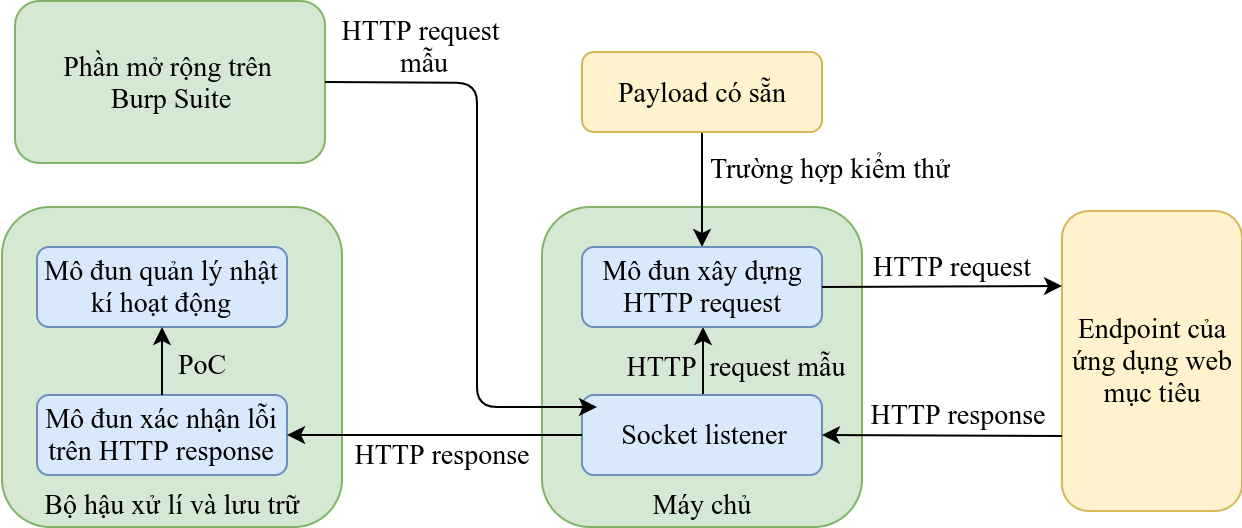
\includegraphics[width=\textwidth,keepaspectratio=true]{images/final-architecture.png}
%   \caption{Kiến trúc hiện thực chính thức của công cụ}
%   \label{fig:final-architecture}
% \end{figure}
% % TODO: Viết thêm về cách xây dựng Burp Suite extension chỗ này 
% Trong quá trình kiểm thử giao diện web bằng tay, sẽ có những \acrshort{http} request được gửi đi thông qua việc gọi đường dẫn URL kèm tham số hoặc việc gửi văn bản, hình ảnh chứa payload đến điểm cuối của ứng dụng web mục tiêu, tương ứng cũng sẽ có những \acrshort{http} response được trả về. Công cụ này sử dụng thêm một phần mở rộng Burp Suite như một proxy trung gian (interception proxy) để giữ lại những \acrshort{http} request thông qua quá trình lựa chọn bằng tay, sau đó chọn ra những tham số cần kiểm thử và chuyển tiếp request mẫu (base request) đó đến mô-đun xây dựng \acrshort{http} request để tiếp tục quá trình kiểm thử với những payload khác. Việc này giúp xác định chính xác điểm cuối cũng như các tham số kèm theo request, ta chỉ việc thay đổi giá trị của các tham số bằng payload khác nhau mà thôi. Việc này cũng giúp loại bỏ nhu cầu thử sai với số lượng rất lớn những điểm cuối và tham số không liên quan (có thể không mắc phải lỗ hổng bảo mật nào), từ đó tăng hiệu năng và giảm thời gian thực thi của công cụ đi rất nhiều.\par
% \textbf{Máy chủ} là bộ phận trung tâm đảm nhiệm chức năng gửi và nhận \acrshort{http} request/response, tương tác với ứng dụng web mục tiêu. Máy chủ này có thể do ta tự triển khai (deploy) hoặc triển khai trên các dịch vụ cung cấp máy chủ ảo hóa (virtual private service - \acrshort{vps} hay virtual dedicated server - VDS) để có thể linh hoạt sử dụng công cụ trước nguy cơ bị chặn bởi địa chỉ IP theo vùng địa lý hoặc bởi các chính sách kiểm soát lưu lượng truy cập của nhà cung cấp ứng dụng web trong tương lai. Bộ phận này gồm có hai mô-đun phụ.
% \begin{itemize}
%     \item \textbf{Mô-đun xây dựng \acrshort{http} request} sẽ dựng nên một \acrshort{http} request hoàn chỉnh bằng cách thay thế payload có sẵn đã được làm rối vào những chỗ được ta đánh dấu. Request sau khi được dựng lên xong sẽ được gửi đến một điểm cuối (endpoint) của ứng dụng web mục tiêu đồng thời được truyền vào mô-đun xác nhận lỗi cũng với \acrshort{http} response tương ứng mà ứng dụng web trả về cho máy chủ để kiểm tra và lưu vào nhật kí hoạt động sau này. Mô-đun này được hiện thực bằng một hàng đợi lần lượt gửi đi các request hoàn chỉnh đã được dựng lại và chèn payload vào.
%     \item \textbf{Mô-đun socket listener} được hiện thực bằng socket sẽ liên tục lắng nghe mọi \acrshort{http} request mẫu và response gửi đến nó và chuyển tiếp response đến mô-đun xác nhận lỗi hoặc chuyển tiếp request mẫu đến mô-đun xây dựng \acrshort{http} request. 
% \end{itemize}
% Nhiều payload cùng mục đích được gom thành các lớp, phục vụ cho việc kiểm thử, đánh giá và so sánh kết quả với các công cụ khác về khả năng phát hiện cùng một lỗ hổng cụ thể. Các trường hợp kiểm thử này sau đó được sử dụng trong bộ kiểm thử giao diện ứng dụng web và máy chủ. Nhiều trường hợp kiểm thử cùng mục đích được gom thành các lớp, phục vụ cho việc kiểm thử, đánh giá và so sánh kết quả với các công cụ khác về khả năng phát hiện cùng một lỗ hổng cụ thể. \par
% \textbf{Bộ hậu xử lí và lưu trữ nhật kí hoạt động} có chức năng xác định việc áp dụng trường hợp kiểm thử trên giao diện web hoặc gửi đến điểm cuối của ứng dụng web mục tiêu có khai thác được lỗ hổng (nếu có) như mong muốn của ta không.
% \begin{itemize}
%     \item \textbf{Mô-đun xác nhận lỗi trên \acrshort{http} response} xử lí lần lượt từng response theo trình tự first-in-first-out. Mô-đun này được hiện thực dựa trên các phương pháp phát hiện lỗ hổng \acrshort{xss}, \acrshort{lfi} và time-based \acrshort{sqli} như đã trình bày ở trên.
%     \item \textbf{Mô-đun quản lý nhật kí hoạt động} sẽ ghi lại trường hợp kiểm thử và \acrshort{poc} chỉ ra rằng việc áp dụng trường hợp kiểm thử đó sẽ khai thác được lỗ hổng nào căn cứ vào các điểm bất thường trên \acrshort{http} response. Mô-đun này sẽ ghi lại những trường hợp kiểm thử và kết quả kiểm tra (đã được mô-đun xác nhận lỗi cho là có lỗ hổng - \texttt{[passed]}) và cả những trường hợp bất thường chưa rõ nguyên nhân (\texttt{[skeptical]}) để hậu kiểm bằng tay.
% \end{itemize}
